\newpage
\section{Other Classifiers}
%\begin{figure}[H]
%  \centering
%  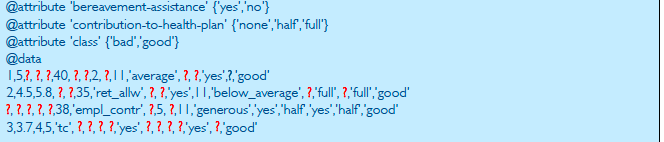
\includegraphics[width=.5\linewidth]{arffmissing}
%\end{figure}

\subsection{Naives Bayes Classifier}
\begin{itemize}
\item \textbf{Conditional probability} :
$$ P(C|A) = \frac{P (A \land C)}{P(A)}$$
$$ P(A|C) = \frac{P (A \land C)}{P(C)}$$
\item Bayes Theorem : 
$$ P(C|A) = \frac{P(A|C)P(C)}{P(A)}$$
\end{itemize}
A \textbf{prior probability} of C , $P(C)$, is the probability of an event before evidence is seen.
A \textbf{posterior probability} of C , $P(C|A)$ , is the probability of an event after evidence is seen.
The probability of a \textbf{class} given an example:
\begin{itemize}
\item A s ample is a  tuple of attributes $$ \overrightarrow{x} = \langle x_1,...,x_n\rangle $$
\item Given target y for the instance , find class with the \textbf{highest probability} for x:
$$ class= arg max _y P(y| \overrightarrow{x})$$
\end{itemize}
Given the target y and sample x described by n attributes ( assumed \textbf{statistically independent) for simplification} , the Bayes Theorem states that:  
$$ P(y|\overrightarrow{x}) = \frac{P(\overrightarrow{x}|y)P(y)}{P(\overrightarrow{x})} = \frac{P(\overrightarrow{x_1}|y)...P(\overrightarrow{x_n}|y)P(y)}{P(\overrightarrow{x})} =$$
\begin{itemize}
\item \textbf{Training}\\
Computes the class probability $P(H)$  and the conditional probability $P(e_i|H)$ for each attribute value $e_i$ and each class H.
\item \textbf{Testing}\\
Given an example E , computes the class:
$$ class = argmax_y P(y|\overrightarrow{x})=\frac{P(\overrightarrow{x_1}|y)...P(\overrightarrow{x_n}|y)P(y)}{P(\overrightarrow{x})} $$
$$ = P(\overrightarrow{x_1}|y)...P(\overrightarrow{x_n}|y)P(y)$$
\end{itemize}
The classifier makes the assumptions that attributes are \textbf{independent} and \textbf{equally important}. Independent means that knowing the value of one attribute says nothing about the value of another : this is \textbf{often not true}! 
Example
\begin{figure}[H]
  \centering
  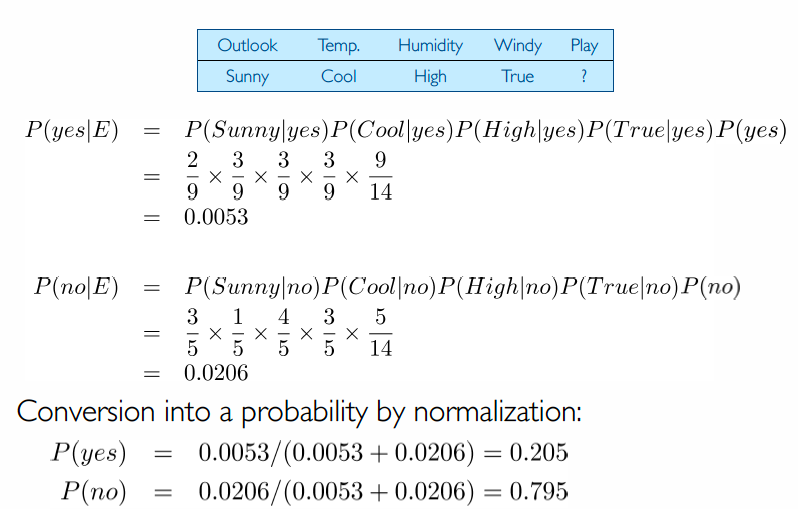
\includegraphics[width=.7\linewidth]{naiveb}
\end{figure}
The \textbf{Zero-Frequency Problem} occurs when  an attribute value does not occur with every class , for example $$ \text{P(humidity = high	}|yes)=0$$
So no matter what the whole probability goes to zero.\\
A solution is to \textbf{add a constant term } to avoid this situation:
\begin{itemize}
\item add \textbf{1} to every count (\textbf{Laplace estimator})
\item add a constant $\neq 1$
\begin{figure}[H]
  \centering
  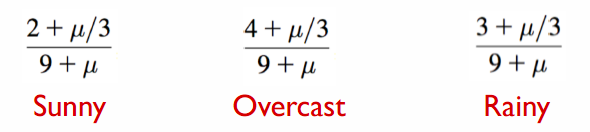
\includegraphics[width=.5\linewidth]{naive2}
\end{figure}
\item add \textbf{weight} (can be different but must sum up to 1)
\begin{figure}[H]
  \centering
  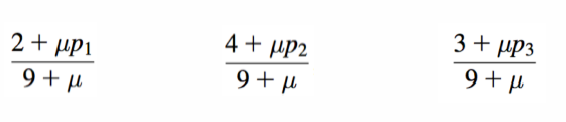
\includegraphics[width=.5\linewidth]{naive3}
\end{figure}
\end{itemize}
A \textbf{missing value} will not be counted during training , and will me \textbf{omitted} during testing .\\
\textbf{Numeric attributes} are assumed to have \textbf{Gaussian} or \textbf{Normal} distribution (given the class). The probability distribution function is defined by \textbf{mean} and \textbf{standard deviation}:
\begin{itemize}
\item \textbf{Sample mean} : $\mu = \frac{1}{n} \sum \limits_{i=1}^{n} x_i$
\item \textbf{Std Deviation} : $\sigma = \frac{1}{n-1} \sum \limits_{i=1}^{N}(x_i - \mu)^2$
\item \textbf{Density function} : $f(x) = \frac{1}{\sqrt{2 \pi \sigma} e^{- \frac{(x-\mu)^2}{2\sigma ^2}}}$
\end{itemize}
However often numeric attributes are \textbf{not normally distributed}.
Also it is not always true that attributes are statistically independent : but this does \textbf{not} affect the performance of such a classifier as its performances are surprisingly good : classification does not require too much precision on probability estimates as long as the \textbf{maximum probability } is assigned correctly to a class.

\subsection{Nearest Neighbour}
Is a kind of \textbf{instance based learning}. A new sample is classified by looking for the k-most similar ones to the given sample and assigning it the majority class: 
\begin{figure}[H]
  \centering
  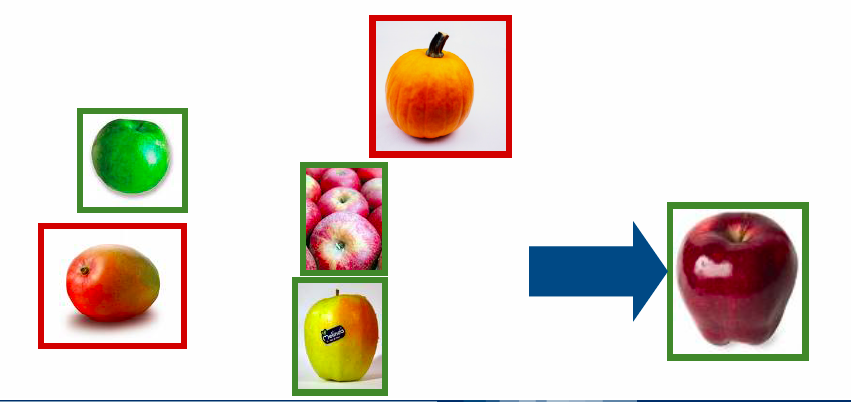
\includegraphics[width=.6\linewidth]{knn}
\end{figure}
Instance based learning does \textbf{not compute} a model, but uses the \textbf{training records} to predict an unknown class label. This methods uses a  \textbf{similarity measure} to define what is learned. K-Nearest-Neighbours implements this kind of instance based learning:
\begin{figure}[H]
  \centering
  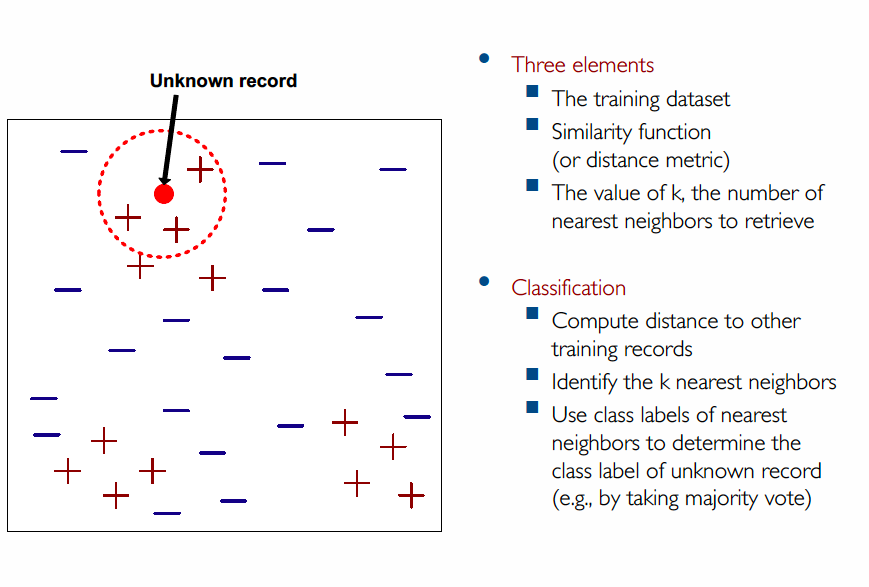
\includegraphics[width=.7\linewidth]{knn2}
\end{figure}
Choosing \textbf{k} correctly is important:
\begin{itemize}
\item \textbf{too small} : classification might be to sensitive to noise points
\item \textbf{too large} : classification might include too dissimilar points
\end{itemize}
Also the choice of the \textbf{similarity measure} is important :
\begin{itemize}
\item \textbf{Euclidean distance}\\
$$ d(p,q) = \sqrt{\sum \limits_i (p_i-q_i)^2}$$
To determine the class from nearest neighbour just take the \textbf{majority vote} class label among the k neighbours or weight the vote according to distance.Other popular Euclidean Distances are:
\begin{itemize}
\item \textbf{Lr Norm} $ (\sum \limits_{i}^{n} |x_i - y_i|^r)^{\frac{1}{r}}$ 
\item \textbf{Manhattan} $(\sum \limits_{i}^{n} |x_i - y_i|$
\item \textbf{L infinite norm} $max_{i=1}^n |x_i-y_i|$
\end{itemize}

\item \textbf{Cosine distance}\\
The cosine distance between x,y is the \textbf{angle} that the vectors to the point make $$ d(\overrightarrow{x},\overrightarrow{y})= arccos \frac{\sum \limits_{i=1}^{n}x_iy_i}{\sqrt{\sum \limits x_i^2}\sqrt{y_i^2}}$$
This angle will be between 0 and 180 no matter how many dimension there are.

\item \textbf{Jaccard distance}\\
Is a measure of how \textbf{dissimilar} two sets are : 
$$ d(\overrightarrow{x},\overrightarrow{y}) = 1-J(\overrightarrow{x},\overrightarrow{y}) $$
$$ J(\overrightarrow{x},\overrightarrow{y}) = \frac{|\overrightarrow{x} \cap \overrightarrow{y}|}{|\overrightarrow{x} \cup \overrightarrow{y}|}$$

\item \textbf{Hamming distance}\\
Hamming distance between two vectors is the number of components in which they differ or equivalently : 
$$ d(\overrightarrow{x},\overrightarrow{y}) = \frac{n-m}{m}$$ where n are the number of variables and m the number of matching components.
 
\end{itemize}
Another important step in KNN is \textbf{normalization} . Attributes are measured on \textbf{different} scales and need to be normalized using :
\begin{itemize}
\item \textbf{Instance range normalisation} : $x_i = \frac{x_i - min_i x_i}{max_i x_i - min_i x_i}$
\item \textbf{standard score normalisation} : $x_i = \frac{x_i - \mu }{\sigma}$ 
\end{itemize}
For nominal attributes the value is 0 if they are not the same value , 1 if they are.\\
Missing values are assumed to \textbf{maximally distant}

\subsubsection{Improving KNN}
KNN can be slow as it requires \textbf{linear scans} of the data.Classification time is proportional to the product of the number of instances.To speed this up there are different techniques like \textbf{KD-Trees}: they split the space hierarchically  using a tree generated from the data. To find a neighbour simply navigate the tree
\begin{figure}[H]
  \centering
  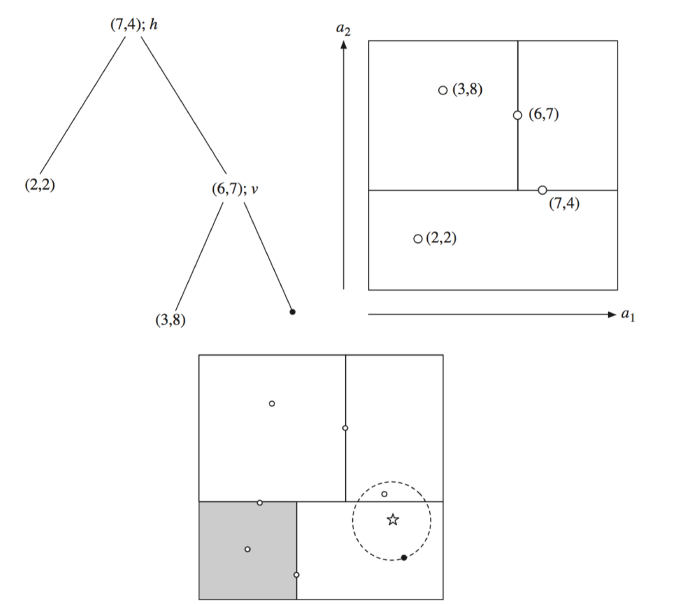
\includegraphics[width=.7\linewidth]{kdtree}
\end{figure}
The tree is navigated
KD Trees \textbf{don't care about the class} , they just partition the space.\\
Complexity depends on the \textbf{depth of the tree},given by the logarithm of number of nodes for a balanced tree.\\
A good KD Tree :
\begin{itemize}
\item  need to find good split and split direction
\item possible split direction where the greatest variance is
\item possible split point on the median value along that direction (mean can be used if data is \textbf{skewed})%
\end{itemize}

\subsubsection{KNN Regression}
KNN can also be used for \textbf{regression} , done in a \textbf{non-parametric} way ( no learning of a model and weights) : KNN fits each point locally and computes the $y_p$ value of a new point $x_p$ by local \textbf{interpolating} the targets associated to neighbour points (prediction can use plain average or weighted average). 

\subsubsection{KNN Discussion}
KNN is often very accurate but also very slow (speed up with KD Trees or Ball Trees). It assumes all attributes are equally important so considering an attribute selection first may improve the performances.\\
In case of \textbf{noisy} instance KNN should be applied using a majority vote over the k-nearest or remove noisy data ( difficult!).

\subsection{Bayesian Belief Networks}
This model doesn't make all the assumptions of Naive Bayes Classifiers:
\begin{itemize}
\item BNN allow to \textbf{specify} which pair of attributes are \textbf{conditionally independent}.
\item BNN provide a method to graphically represent \textbf{probabilistic relationships} among a set of variables
\end{itemize}
BNN describe the probability distribution governing a set of variables by using \textbf{conditional independence} assumptions on a subsets of variables and a set of \textbf{conditional probabilities}.
So what is needed :
\begin{itemize}
\item \textbf{Acylic Graph} = encodes the relationships among variables
\item \textbf{Probability table} = associating each node to its immediate parent node
\end{itemize}
\begin{figure}[H]
  \centering
  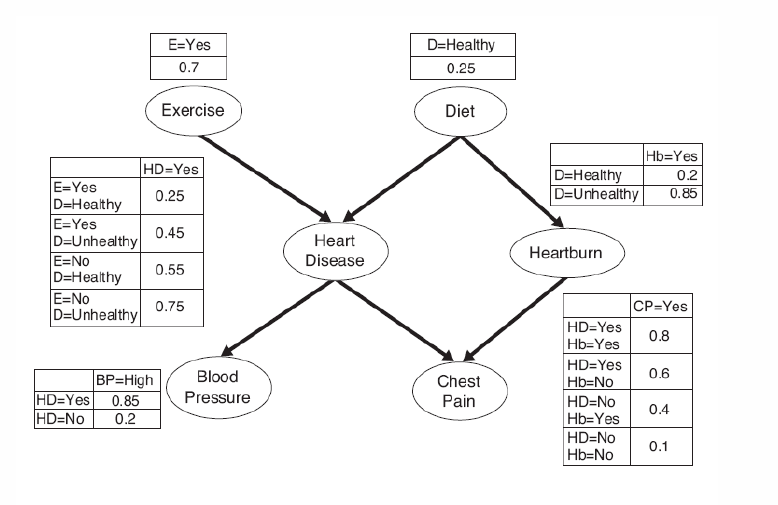
\includegraphics[width=.7\linewidth]{belief}
\end{figure}
\begin{itemize}
\item If a node does not have a parent is contains the \textbf{prior probability} P(X) (like Exercise and Diet)
\item If a node has just one parent it contains the conditional probability $P(X|Y)$
\item If a node has more parents it contains the conditional probability $PX|Y_1,...,Y_k$ 
\end{itemize}
BNN are very useful to incorporate \textbf{domain knowledge} into the model (other model cannot do this!). BNN's are very time consuming but adding variables is very easy. They are robust to overfitting and also work on incomplete data.

\subsection{Support Vector Machines}
Two classes can be separated in many ways : SVMs work by \textbf{maximizing} the margin :
\begin{figure}[H]
  \centering
  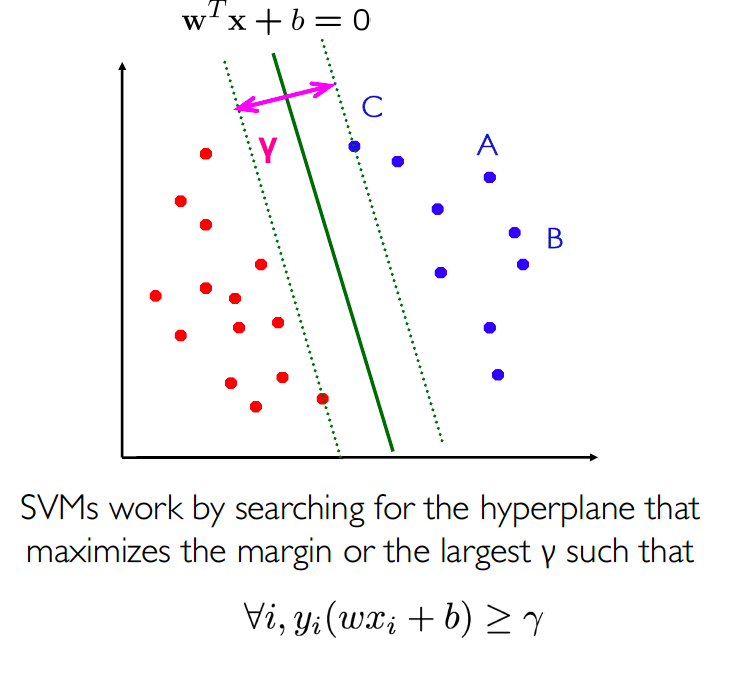
\includegraphics[width=.7\linewidth]{svm}
\end{figure}